\chapter{Two Sample Hypothesis Tests}

%%%%%%%%%%%%%%
%%% Nurlana's work %%%
%%%%%%%%%%%%%%

\section{Comparing Means with Independent Samples}
\begin{figure}[H]
\centering
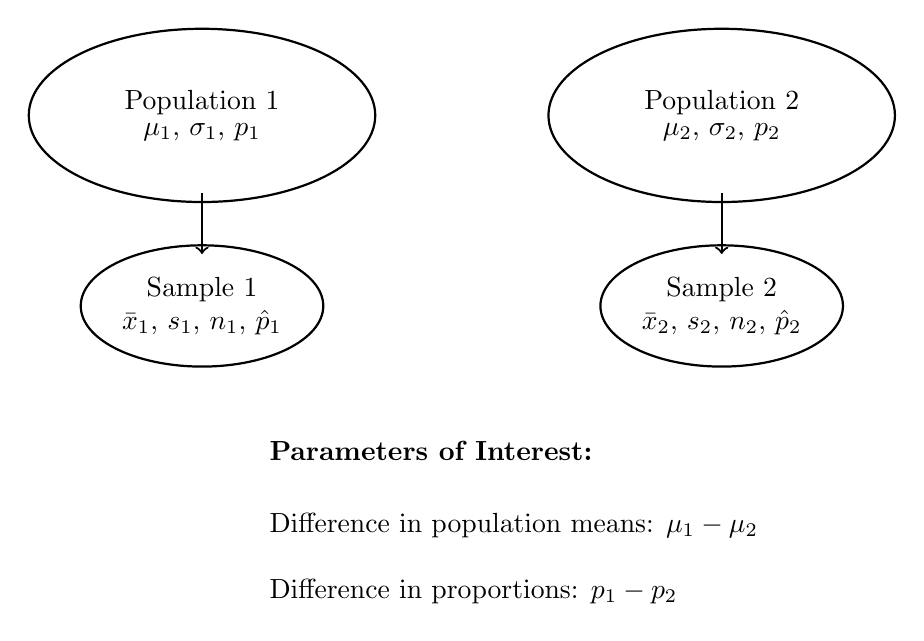
\begin{tikzpicture}[scale=1.1]

% Population 1
\draw[thick] (0,3.5) ellipse (2 and 1);
\node at (0,3.5) {\shortstack{Population 1 \\ $\mu_1$, $\sigma_1$, $p_1$}};

% Sample 1
\draw[thick] (0,1.3) ellipse (1.4 and 0.7);
\node at (0,1.3) {\shortstack{Sample 1 \\ $\bar{x}_1$, $s_1$, $n_1$, $\hat{p}_1$}};

% Arrow from Pop1 to Sample1
\draw[->, thick] (0,2.6) -- (0,1.9);

% Population 2
\draw[thick] (6,3.5) ellipse (2 and 1);
\node at (6,3.5) {\shortstack{Population 2 \\ $\mu_2$, $\sigma_2$, $p_2$}};

% Sample 2
\draw[thick] (6,1.3) ellipse (1.4 and 0.7);
\node at (6,1.3) {\shortstack{Sample 2 \\ $\bar{x}_2$, $s_2$, $n_2$, $\hat{p}_2$}};

% Arrow from Pop2 to Sample2
\draw[->, thick] (6,2.6) -- (6,1.9);

% Parameters of Interest
\node[align=left] at (3.6,-1.2) {
\textbf{Parameters of Interest:} \\\\[2pt]
Difference in population means: $\mu_1 - \mu_2$ \\\\
Difference in proportions: $p_1 - p_2$
};

\end{tikzpicture}
\caption{Structure of Two-Sample Hypothesis Tests}
\end{figure}
\subsection*{Setting Up Hypotheses}

Let $\theta_1$ and $\theta_2$ be the parameters of interest from populations 1 and 2, respectively.

\vspace{0.8em}
\noindent\textbf{1. Interested in whether $\theta_1 > \theta_2$:}
\begin{align*}
H_0\!:~ & \theta_1 = \theta_2 \\
H_a\!:~ & \theta_1 > \theta_2 \\
\text{Equivalent:} \quad & H_0\!:~ \theta_1 - \theta_2 = 0 \qquad H_a\!:~ \theta_1 - \theta_2 > 0
\end{align*}

\vspace{0.8em}
\noindent\textbf{2. Interested in whether $\theta_1 < \theta_2$:}
\begin{align*}
H_0\!:~ & \theta_1 = \theta_2 \\
H_a\!:~ & \theta_1 < \theta_2 \\
\text{Equivalent:} \quad & H_0\!:~ \theta_1 - \theta_2 = 0 \qquad H_a\!:~ \theta_1 - \theta_2 < 0
\end{align*}

\vspace{0.8em}
\noindent\textbf{3. Interested in whether $\theta_1 \ne \theta_2$:}
\begin{align*}
H_0\!:~ & \theta_1 = \theta_2 \\
H_a\!:~ & \theta_1 \ne \theta_2 \\
\text{Equivalent:} \quad & H_0\!:~ \theta_1 - \theta_2 = 0 \qquad H_a\!:~ \theta_1 - \theta_2 \ne 0
\end{align*}
\subsection*{Structure of a Test Statistic}

\noindent
The general structure of a test statistic is:
\[
\text{test statistic} = \frac{\text{(observed statistic)} - \text{(hypothesized value)}}{\text{standard error}}
\]

\bigskip
\noindent\textbf{Common Cases:}
\begin{itemize}
  \item $\sigma$ known: \quad $z = \dfrac{\bar{x} - \mu_0}{\sigma / \sqrt{n}}$
  \item $\sigma$ unknown: \quad $t = \dfrac{\bar{x} - \mu_0}{s / \sqrt{n}}$
  \item Proportions: \quad $z = \dfrac{\hat{p} - p_0}{\sqrt{p_0(1 - p_0)/n}}$
\end{itemize}
\section*{Hypothesis Test on a Difference of Means (\texorpdfstring{$\mu_1 - \mu_2$}{mu1 - mu2})}
\begin{itemize}
\item When $\sigma_1$ and $\sigma_2$ are known:
\end{itemize}
\begin{align*}
H_0&: \mu_1 - \mu_2 = 0 \\
H_a&: \mu_1 - \mu_2 > 0 \quad \text{(or } < 0 \text{, } \ne 0 \text{)}
\end{align*}

\textbf{Test Statistic:}
\[
z = \frac{(\bar{x}_1 - \bar{x}_2) - 0}{\sqrt{\frac{\sigma_1^2}{n_1} + \frac{\sigma_2^2}{n_2}}}
\]

Reference distribution: standard normal (Z distribution).

\textit{Note: This scenario is rare in practice since both population standard deviations $\sigma_1$ and $\sigma_2$ are seldom known.}
\vspace{0.5em}
\begin{itemize}
\item When $\sigma_1$ and $\sigma_2$ are unknown: 
\end{itemize}
\vspace{1.0em}
\textbf{Case 1: Assume equal variances $\sigma_1^2 = \sigma_2^2$}
\vspace{0.5em}
\begin{align*}
H_0&: \mu_1 - \mu_2 = 0 \\
H_a&: \mu_1 - \mu_2 > 0 \quad \text{(or } < 0 \text{, } \ne 0 \text{)}
\end{align*}

\textbf{Test Statistic:}
\[
t = \frac{(\bar{x}_1 - \bar{x}_2) - 0}{s_p \sqrt{\frac{1}{n_1} + \frac{1}{n_2}}}
\]

where the pooled standard deviation is defined as:
\[
s_p^2 = \frac{(n_1 - 1)s_1^2 + (n_2 - 1)s_2^2}{n_1 + n_2 - 2}
\]

Reference distribution: $t$-distribution with $n_1 + n_2 - 2$ degrees of freedom.

(Use this only when equal variances can reasonably be assumed.) \\
\vspace{1.0em}

\noindent \textbf{Case 2: Assume Unequal Variances $\sigma_1^2 \ne \sigma_2^2$ (Welch's t-test)}
\vspace{0.5em}
\begin{align*}
H_0 &: \mu_1 - \mu_2 = 0 \\
H_a &: \mu_1 - \mu_2 > 0 \quad (\text{or } < 0,\ \ne 0)
\end{align*}

\textbf{Test Statistic:}
\[
t^* = \frac{(\bar{x}_1 - \bar{x}_2) - 0}{\sqrt{\frac{s_1^2}{n_1} + \frac{s_2^2}{n_2}}}
\]

Reference distribution: approximately a $t$-distribution.

\vspace{0.5em}
\textit{Degrees of freedom (by hand):}
\[
\min(n_1 - 1,\ n_2 - 1)
\]

\textit{Note:} R uses a more sophisticated approximation for degrees of freedom in this case.
\section*{Comparing Means of Independent Samples (Normal Population Assumptions)}

We should check the assumption that the underlying populations of individual responses are each Normally distributed. Nearly Normal Condition:

\begin{itemize}
  \item We must check this for both groups; a violation for either one violates the condition.
  \item The Normality assumption matters most when sample sizes are very small.
  \item For $n < 10$ in either group, this method should not be used if the histogram or Normality plots show clear skewness.
  \item For $n$’s of 10 or so, a moderately skewed histogram is okay. But, for strongly skewed data or data containing outliers this method should be avoided.
  \item For larger samples $n \geq 20$, data skewness is less of an issue — but, we still need to check if there are any outliers in the data, extreme skewness, and multiple modes.
\end{itemize}
\subsection{Comparing Two Populations Means: Independent Sampling (Equal Variances Assumed)}

Consider two independent populations with unknown means $\mu_1$ and $\mu_2$, and unknown standard deviations $\sigma_1$ and $\sigma_2$ ($\sigma_1 = \sigma_2$), respectively. We can make an inference about their mean difference $\mu_1 - \mu_2$ by using the difference between their point estimates (sample means): $\bar{Y}_1 - \bar{Y}_2$. When the assumptions and conditions are met,

\[
\frac{(\bar{Y}_1 - \bar{Y}_2) - (\mu_1 - \mu_2)}{S_p \sqrt{\frac{1}{n_1} + \frac{1}{n_2}}}
= \frac{(\bar{Y}_1 - \bar{Y}_2) - (\mu_1 - \mu_2)}{\sqrt{S_p^2 \left[\frac{1}{n_1} + \frac{1}{n_2} \right] }},
\]

can be modelled by a $t(\nu)$ distribution; where $\nu = n_1 + n_2 - 2$ and

\[
S_p^2 = \frac{(n_1 - 1)s_1^2 + (n_2 - 1)s_2^2}{n_1 + n_2 - 2}.
\]
\begin{tcolorbox}[
  colback=yellow!5,
  colframe=yellow!50!black,
  title={Comparing Two Populations Means: Independent Sampling (Equal Variances Assumed) (cont.)},
  sharp corners,
  boxrule=0.4pt,
  width=\textwidth,
  breakable
]

\textbf{Conditions Required for Valid Inference about $\mu_1 - \mu_2$:}

\begin{enumerate}
  \item The two samples are randomly selected in an independent manner from the two target populations.
  \item Both sampled populations have distributions that are approximately Normal.
  \item The population variances are equal (e.g., $\sigma_1 = \sigma_2$).
\end{enumerate}
\end{tcolorbox}
\subsection*{Small-Sample Confidence Interval for $\mu_1 - \mu_2$ (with equal variances)}

\textbf{Parameter:} $\mu_1 - \mu_2$

\vspace{0.5em}

\textbf{Confidence interval} ($\nu = \text{df}$):

\[
(\bar{Y}_1 - \bar{Y}_2) \pm t_{\alpha/2}(\nu) S_p \sqrt{\frac{1}{n_1} + \frac{1}{n_2}},
\]

where $\nu = n_1 + n_2 - 2$ and
\[
S_p^2 = \frac{(n_1 - 1)s_1^2 + (n_2 - 1)s_2^2}{n_1 + n_2 - 2}
\]

(requires that Normal samples are independent and the assumption that $\sigma_1^2 = \sigma_2^2$). The critical value $t_{\alpha/2}(\nu)$ depends on the particular confidence level and the number of degrees of freedom.
\begin{example}
Comparing Two Population Means Managerial Success Indexes for Two Groups (With Equal Variances Assumed)

Behavioural researchers have developed an index designed to measure managerial success. The index (measured on a 100-point scale) is based on the manager’s length of time in the organization and their level within the term; the higher the index, the more successful the manager. Suppose a researcher wants to compare the average index for the two groups of managers at a large manufacturing plant. Managers in group 1 engage in \textbf{high volume of interactions} with people outside the managers’ work unit (such interaction include phone and face-to-face meetings with customers and suppliers, outside meetings, and public relation work). Managers in group 2 \textbf{rarely interact} with people outside their work unit. Independent random samples of 12 and 15 managers are selected from groups 1 and 2, respectively, and success index of each is recorded.

\vspace{1em}

\textbf{Response variable:} Managerial Success Indexes (quantitative, continuous, 0–100 scale)

\textbf{Explanatory variable:} Type of group (nominal categorical: \textit{Group 1 = interaction with outsiders}, \textit{Group 2 = fewer interactions}) 

\vspace{1em}
\noindent\textbf{R Code}
\begin{tcolorbox}[colback=gray!10, colframe=black!45, arc=2mm,
  before skip=4pt, after skip=4pt]
\begin{verbatim}
# Importing data file into R
success = read.csv(file = "success.csv", header = TRUE);

# Getting names of variables
names(success);

# Seeing first few observations
head(success);

# Attaching data file
attach(success);
\end{verbatim}
\end{tcolorbox}

\noindent\textbf{R Code}
\begin{tcolorbox}[colback=gray!10, colframe=black!45, arc=2mm,
  before skip=4pt, after skip=4pt]
\begin{verbatim}
## [1] "Success_Index" "Group"
##   Success_Index Group
## 1            65     1
## 2            66     1
## 3            58     1
## 4            70     1
## 5            78     1
## 6            53     1
\end{verbatim}
\end{tcolorbox}
\noindent\textbf{R code (Descriptive Statistics)}
\begin{tcolorbox}[colback=gray!10, colframe=black!45, arc=2mm,
  before skip=4pt, after skip=4pt]
\begin{verbatim}
# loading library mosaic
library(mosaic)

favstats(Success_Index ~ Group)
\end{verbatim}
\end{tcolorbox}

\noindent\textbf{R Code (Descriptive Statistics)}
\begin{tcolorbox}[colback=gray!10, colframe=black!45, arc=2mm,
  before skip=4pt, after skip=4pt]
\begin{verbatim}
## .group min   Q1 median   Q3 max     mean       sd  n
##       1  53 62.25  65.50 69.25  78 65.33333 6.610368 12
##       2  34 42.50  50.00 54.50  68 49.46667 9.334014 15
\end{verbatim}
\end{tcolorbox}

\noindent\textbf{R Code (Descriptive Statistics)}
\begin{tcolorbox}[colback=gray!10, colframe=black!45, arc=2mm,
  before skip=4pt, after skip=4pt]
\begin{verbatim}
summary(Success_Index[Group == 1]);
length(Success_Index[Group == 1]);
sd(Success_Index[Group == 1]);

summary(Success_Index[Group == 2]);
length(Success_Index[Group == 2]);
sd(Success_Index[Group == 2]);
\end{verbatim}
\end{tcolorbox}

Note: Group 1 = “interaction with outsiders” and Group 2 = “fewer interactions”.
% --- continuation inside the same example environment ---

\noindent\textbf{R Output}
\begin{tcolorbox}[colback=gray!10, colframe=black!45, arc=2mm,
  before skip=4pt, after skip=4pt]
\begin{verbatim}
##  Min.  1st Qu.  Median    Mean  3rd Qu.    Max. 
##  53.00   62.25   65.50   65.33   69.25   78.00 
## [1] 12
## [1] 6.610368

##  Min.  1st Qu.  Median    Mean  3rd Qu.    Max. 
##  34.00   42.50   50.00   49.47   54.50   68.00 
## [1] 15
## [1] 9.334014
\end{verbatim}
\end{tcolorbox}

\vspace{0.5em}
\noindent\textbf{Nearly Normal Condition (Group 1: “interaction with outsiders”):}
\begin{tcolorbox}[colback=gray!10, colframe=black!45, arc=2mm,
  before skip=4pt, after skip=4pt]
\begin{verbatim}
stem(Success_Index[Group == 1]);
\end{verbatim}
\end{tcolorbox}

\noindent\textbf{R Output}
\begin{tcolorbox}[colback=gray!10, colframe=black!45, arc=2mm,
  before skip=4pt, after skip=4pt]
\begin{verbatim}
## 
##  The decimal point is 1 digit(s) to the right of the |
## 
##  5 | 38
##  6 | 0335689
##  7 | 018
\end{verbatim}
\end{tcolorbox}

\vspace{0.5em}
\noindent\textbf{Nearly Normal Condition (Group 2: “fewer interactions”):}
\begin{tcolorbox}[colback=gray!10, colframe=black!45, arc=2mm,
  before skip=4pt, after skip=4pt]
\begin{verbatim}
stem(Success_Index[Group == 2]);
\end{verbatim}
\end{tcolorbox}

\noindent\textbf{R Output}
\begin{tcolorbox}[colback=gray!10, colframe=black!45, arc=2mm,
  before skip=4pt, after skip=4pt]
\begin{verbatim}
## 
##  The decimal point is 1 digit(s) to the right of the |
## 
##  3 | 46
##  4 | 22368
##  5 | 023367
##  6 | 28
\end{verbatim}
\end{tcolorbox}

\vspace{0.5em}
\noindent\textbf{Nearly Normal Condition (Group 1: “interaction with outsiders”):}
\begin{tcolorbox}[colback=gray!10, colframe=black!45, arc=2mm,
  before skip=4pt, after skip=4pt]
\begin{verbatim}
qqnorm(Success_Index[Group == 1]);
qqline(Success_Index[Group == 1]);
\end{verbatim}
\end{tcolorbox}
\begin{figure}[H]
\centering
\includegraphics[width=0.6\textwidth]{section14.1/images/qqplot_group1.pdf}
\caption{Q-Q Plot for Group 1: Interaction with Outsiders}
\label{fig:qqplot-group1}
\end{figure}
\vspace{0.5em}
\noindent\textbf{Nearly Normal Condition (Group 2: “fewer interactions”):}
\begin{tcolorbox}[colback=gray!10, colframe=black!45, arc=2mm,
  before skip=4pt, after skip=4pt]
\begin{verbatim}
qqnorm(Success_Index[Group == 2]);
qqline(Success_Index[Group == 2]);
\end{verbatim}
\end{tcolorbox}
\noindent
\begin{minipage}{\textwidth}
\centering
\includegraphics[width=0.6\textwidth]{section14.1/images/qqplot_group2.pdf}
\vspace{-0.5em}

\captionof{figure}{Q-Q Plot for Group 2: Fewer Interactions}
\label{fig:qqplot-group2}
\end{minipage}

\vspace{1.00em}

\noindent\textbf{Nearly Normal Condition:}
\begin{tcolorbox}[colback=gray!10, colframe=black!45, arc=2mm,
  before skip=4pt, after skip=4pt]
\begin{verbatim}
boxplot(Success_Index ~ Group, col = c("red", "blue"))
\end{verbatim}
\end{tcolorbox}
\noindent
\begin{minipage}{\textwidth}
\centering
\includegraphics[width=0.55\textwidth]{section14.1/images/boxplot_success_index.pdf}
\vspace{-0.5em}

\captionof{figure}{Boxplot of Success Index by Group}
\label{fig:boxplot-success}
\end{minipage}
\vspace{-1,00em}

\noindent\textbf{Boxplot with \texttt{ggplot2}:}
\begin{tcolorbox}[colback=gray!10, colframe=black!45, arc=2mm,
  before skip=4pt, after skip=4pt]
\begin{verbatim}
# loading library;
library(ggplot2);

# converting a numeric variable into factor (categorical data)
group <- factor(Group);

# bp: just a name (not code) to store boxplots;
bp <- ggplot(success,
             aes(x = group, y = Success_Index, fill = group));

our.labs <- c("Interaction with Outsiders", "Fewer Interactions");

bp +
  geom_boxplot() +
  scale_x_discrete(labels = our.labs);
\end{verbatim}
\end{tcolorbox}
\begin{figure}[H]
\centering
\includegraphics[width=0.6\textwidth]{section14.1/images/boxplot_ggplot2.pdf}
\caption{Boxplot of Success Index by Group using ggplot2}
\label{fig:boxplot-ggplot}
\end{figure}
\noindent\textbf{Checking the Assumptions and Conditions}

\vspace{0.5em}

\noindent\textbf{Independent Group Assumption:} The success index in group 1 is unrelated to the success index in group 2.

\noindent\textbf{Randomization Condition:} The 27 managers were randomly and independently selected (12 for group 1, and 15 for group 2).

\noindent\textbf{Nearly Normal Condition:} The two boxplots of success indexes do not show skewness; the two stemplots/histograms of success indexes are unimodal, fairly symmetric and approximately bell-shaped. Q–Q plots also suggest the normality assumption is reasonable.

\noindent\textbf{Equal Variances Assumption:} The two boxplots of success indexes appear to have the same spread; thus, the samples appear to have come from populations with approximately the same variance.

\vspace{0.5em}

Since the conditions are satisfied, it is appropriate to construct a $t$ confidence interval with\\
$df = 12 + 15 - 2 = 25$. \\

\noindent\textbf{From the data, the following statistics were calculated:}

\[
\begin{aligned}
n_1 &= 12 &\quad n_2 &= 15 \\
\bar{x}_1 &= 65.33 &\quad \bar{x}_2 &= 49.47 \\
s_1^2 &= 6.61^2 &\quad s_2^2 &= 9.33^2
\end{aligned}
\]

\vspace{1em}
\noindent\textbf{The pooled variance estimator is:}

\[
s_p^2 = \frac{(n_1 - 1)s_1^2 + (n_2 - 1)s_2^2}{n_1 + n_2 - 2} 
= \frac{(12 - 1)(6.61^2) + (15 - 1)(9.33^2)}{12 + 15 - 2}
= 67.97
\]

\vspace{1em}
\noindent\textbf{The number of degrees of freedom is:}
\[
\nu = n_1 + n_2 - 2 = 12 + 15 - 2 = 25
\]

\vspace{1em}
\noindent\textbf{Two-sample t-test (Student’s t-test) for the Difference Between Means $\mu_1 - \mu_2$:}

Is there evidence to suggest that the mean success index differs between the two groups?

\vspace{1em}
\noindent\textbf{1. State Hypotheses:}
\[
\begin{aligned}
H_0 &: \mu_1 = \mu_2 \quad \text{or} \quad H_0 : \mu_1 - \mu_2 = 0 \\
H_a &: \mu_1 \ne \mu_2 \quad \text{or} \quad H_a : \mu_1 - \mu_2 \ne 0
\end{aligned}
\]

\vspace{1em}
\noindent\textbf{2. Test Statistic:}
\[
t^* = \frac{\bar{x}_1 - \bar{x}_2}{\sqrt{\frac{s_p^2}{n_1} + \frac{s_p^2}{n_2}}}
= \frac{65.33 - 49.47}{\sqrt{\frac{67.97}{12} + \frac{67.97}{15}}}
= 4.97
\]

\vspace{1em}
\noindent\textbf{3. P-value:}

Using table:
\[
\text{df} = 25 \quad \Rightarrow \quad \text{P-value} < 2(0.005)
\]

Using R:
\begin{tcolorbox}[colback=gray!10, colframe=black!45, arc=2mm, before skip=4pt, after skip=4pt]
\begin{verbatim}
# One way:
2*(1 - pt(4.97, df = 25));

# Another way:
2 * pt(4.97, df = 25, lower.tail = FALSE);
\end{verbatim}
\end{tcolorbox}

Both methods return:
\[
\text{P-value} \approx 4.03 \times 10^{-5}
\]
\vspace{1em}
\noindent\textbf{4. Conclusion.}

Since the P-value is very small, we have strong evidence to indicate that there is a difference in mean success index between group~1 and group~2.

\vspace{0.5em}
\noindent\textbf{Note.} As a follow-up, we could find a 95\% CI for $\mu_1 - \mu_2$ to estimate this difference. Then, we could provide an estimate of how much higher the mean success index for group~1 is.

\end{example}
\subsection{Comparing Two Populations Means: Independent Sampling (Unequal Variances Assumed)}
\subsection*{Small-Sample Confidence Interval for $\mu_1 - \mu_2$ (Unequal Variances)}

Draw an SRS of size $n_1$ from a Normal population with unknown mean $\mu_1$, and draw an independent SRS of size $n_2$ from another Normal population with unknown mean $\mu_2$. A confidence interval for $\mu_1 - \mu_2$ is given by

\[
(\bar{x}_1 - \bar{x}_2) \pm t^* \sqrt{\frac{s_1^2}{n_1} + \frac{s_2^2}{n_2}}
\]

Here $t^*$ is the critical value for the $t(k)$ density curve with area $C$ between $-t^*$ and $t^*$. The degrees of freedom $k$ are equal to the smaller of $n_1 - 1$ and $n_2 - 1$.
\subsection*{Degrees of Freedom}

\textit{Option 1.} With software, use the statistic $t$ with accurate critical values from the approximating $t$ distribution.

The distribution of the two-sample $t$ statistic is very close to the $t$ distribution with degrees of freedom $df$ given by

\[
df = \frac{\left( \frac{s_1^2}{n_1} + \frac{s_2^2}{n_2} \right)^2}
{
\left( \frac{1}{n_1 - 1} \left( \frac{s_1^2}{n_1} \right)^2 \right)
+
\left( \frac{1}{n_2 - 1} \left( \frac{s_2^2}{n_2} \right)^2 \right)
}
\]

This approximation is accurate when both sample sizes $n_1$ and $n_2$ are 5 or larger.
\vspace{0.5em}

\textit{Option 2.} Without software, use the statistic $t$ with critical values from the $t$ distribution with degrees of freedom equal to the smaller of $n_1 - 1$ and $n_2 - 1$. These procedures are always conservative for any two Normal populations.
\subsection*{Two-Sample t-Test (Unequal Variances)}

To test the hypothesis $H_0 : \mu_1 = \mu_2$, calculate the two-sample $t$ statistic:

\[
t^* = \frac{\bar{x}_1 - \bar{x}_2}{\sqrt{\frac{s_1^2}{n_1} + \frac{s_2^2}{n_2}}}
\]

and use $P$-values or critical values for the $t(k)$ distribution.
\begin{example}[Logging in the rain forest]
“Conservationists have despaired over destruction of tropical rain forest by logging, clearing, and burning”. These words begin a report on a statistical study of the effects of logging in Borneo. Here are data on the number of tree species in 12 unlogged forest plots and 9 similar plots logged 8 years earlier:

Unlogged: 22 18 22 20 15 21 13 13 19 13 19 15  \\
Logged : 17 4 18 14 18 15 15 10 12  

Does logging significantly reduce the mean number of species in a plot after 8 years? State the hypotheses and do a t test. Is the result significant at the 5\% level?\\
\vspace{0.5em}
\noindent\textbf{Solution:} \\
1. State hypotheses. $H_0: \mu_1 = \mu_2$ vs.\ $H_a: \mu_1 > \mu_2$, where $\mu_1$ is the mean number of species in unlogged plots and $\mu_2$ is the mean number of species in plots logged 8 years earlier.

2. Test statistic. 
\[
t^* \;=\;\frac{\bar x_1 - \bar x_2}{\sqrt{s_1^2/n_1 + s_2^2/n_2}}
\;=\;2.1140
\]
\[
(\bar x_1 = 17.5,\;\bar x_2 = 13.6666,\;s_1 = 3.5290,\;s_2 = 4.5,\;n_1 = 12,\;n_2 = 9)
\]

3. P-value. Using Table, we have $df = 8$, and $0.025 < \text{P-value} < 0.05$.

4. Conclusion. Since P-value $< 0.05$, we reject $H_0$. There is strong evidence that the mean number of species in unlogged plots is greater than that for logged plots 8 years after logging.
\end{example}
\begin{example}
A company that sells educational materials reports statistical studies to convince customers that its materials improve learning. One new product supplies ``directed reading activities'' for classroom use. These activities should improve the reading ability of elementary school pupils.

A consultant arranges for a third-grade class of 21 students to take part in these activities for an eight-week period. A control classroom of 23 third-graders follows the same curriculum without the activities. At the end of the eight weeks, all students are given a Degree of Reading Power (DRP) test, which measures the aspects of reading ability that the treatment is designed to improve. The data appear in the following table.

\begin{center}
\begin{tabular}{cccccccc}
\toprule
\multicolumn{4}{c}{\textbf{Treatment}} & \multicolumn{4}{c}{\textbf{Control}} \\
\midrule
24 & 61 & 59 & 46 & 42 & 33 & 46 & 37 \\
43 & 44 & 52 & 43 & 43 & 41 & 10 & 42 \\
58 & 67 & 62 & 57 & 55 & 19 & 17 & 55 \\
71 & 49 & 54 &    & 26 & 54 & 60 & 28 \\
43 & 53 & 57 &    & 62 & 20 & 53 & 48 \\
49 & 56 & 33 &    & 37 & 85 & 42 &    \\
\bottomrule
\end{tabular}
\end{center}

Because we hope to show that the treatment (Group 1) is better than the control (Group 2), the hypotheses are:

\[H_0 : \mu_1 = \mu_2\]
\[H_a : \mu_1 > \mu_2\]

\begin{tcolorbox}[colback=gray!10, colframe=black!45, arc=2mm, before skip=4pt, after skip=4pt]
\begin{verbatim}
# Step 1. Entering data
treatment = c(24, 61, 59, 46, 43, 44, 52, 43, 58, 67, 62, 57, 
              71, 49, 54, 43, 53, 57, 49, 56, 33);
control = c(42, 33, 46, 37, 43, 41, 10, 42, 55, 19, 17, 55, 
            26, 54, 60, 28, 62, 20, 53, 48, 37, 85, 42);
\end{verbatim}
\end{tcolorbox}
\noindent\textbf{Nearly Normal Condition (treatment):}
\begin{tcolorbox}[colback=gray!10, colframe=black!45, arc=2mm, before skip=4pt, after skip=4pt]
\begin{verbatim}
# Making stemplot;

stem(treatment);
\end{verbatim}
\end{tcolorbox}
\begin{tcolorbox}[colback=gray!10, colframe=black!45, arc=2mm, before skip=4pt, after skip=4pt]
\begin{verbatim}
##
## The decimal point is 1 digit(s) to the right of the |
##
## 2 | 4
## 3 | 3
## 4 | 3334699
## 5 | 23467789
## 6 | 127
## 7 | 1
\end{verbatim}
\end{tcolorbox}
\noindent\textbf{Nearly Normal Condition (control):}
\begin{tcolorbox}[colback=gray!10, colframe=black!45, arc=2mm, before skip=4pt, after skip=4pt]
\begin{verbatim}
# Making stemplot;

stem(control);
\end{verbatim}
\end{tcolorbox}

\begin{tcolorbox}[colback=gray!10, colframe=black!45, arc=2mm, before skip=4pt, after skip=4pt]
\begin{verbatim}
##
## The decimal point is 1 digit(s) to the right of the |
##
## 0 | 079
## 2 | 068377
## 4 | 12223683455
## 6 | 02
## 8 | 5
\end{verbatim}
\end{tcolorbox}
\noindent\textbf{Nearly Normal Condition (treatment):}
\begin{tcolorbox}[colback=gray!10, colframe=black!45, arc=2mm, before skip=4pt, after skip=4pt]
\begin{verbatim}
# Making Q-Q plot;
qqnorm(treatment, pch=19, col="red", main="Treatment");
qqline(treatment, lty=2);
\end{verbatim}
\end{tcolorbox}
\begin{figure}[H]
\centering
\includegraphics[width=0.6\textwidth]{section14.1/images/treatment_qqplot.pdf}
\caption{Q-Q Plot for Treatment Group}
\label{fig:qqplot-ggplot}
\end{figure}
\noindent\textbf{Nearly Normal Condition (control):}
\begin{tcolorbox}[colback=gray!10, colframe=black!45, arc=2mm, before skip=4pt, after skip=4pt]
\begin{verbatim}
# Making Q-Q plot;
qqnorm(treatment, pch=19, col="red", main="Control");
qqline(control, lty=2);
\end{verbatim}
\end{tcolorbox}
\noindent
\begin{minipage}{\textwidth}
\centering
\includegraphics[width=0.6\textwidth]{section14.1/images/control_qqplot.pdf}
\vspace{-0.5em}

\captionof{figure}{Q-Q Plot for Control Group}
\label{fig:qqplot-ggplot}
\end{minipage}

\vspace{1.00em}
Stemplots suggest that there is a mild outlier in the control group but no deviation from Normality serious enough to prevent us from using t procedures. Normal Q-Q plots for both groups confirm that both are roughly Normal. The summary statistics are:
\begin{tcolorbox}[colback=gray!10, colframe=black!45, arc=2mm, before skip=4pt, after skip=4pt]
\begin{verbatim}
summary(treatment);

## Min. 1st Qu.  Median    Mean 3rd Qu.    Max. 
## 24.00   44.00   53.00   51.48   58.00   71.00

summary(control);

## Min. 1st Qu.  Median    Mean 3rd Qu.    Max. 
## 10.00   30.50   42.00   41.52   53.50   85.00
\end{verbatim}
\end{tcolorbox}

\begin{tcolorbox}[colback=gray!10, colframe=black!45, arc=2mm, before skip=4pt, after skip=4pt]
\begin{verbatim}
# Step 1. Entering data;

treatment = c(24, 61, 59, 46, 43, 44, 52, 43, 58, 67, 62, 57, 
              71, 49, 54, 43, 53, 57, 49, 56, 33);
              
control = c(42, 33, 46, 37, 43, 41, 10, 42, 55, 19, 17, 55, 
            26, 54, 60, 28, 62, 20, 53, 48, 37, 85, 42);

# Step 2. Hypothesis Test

t.test(treatment, control, alternative="greater")
\end{verbatim}
\end{tcolorbox}
\noindent\textbf{HT (using R)}
\begin{tcolorbox}[colback=gray!10, colframe=black!45, arc=2mm, before skip=4pt, after skip=4pt]
\begin{verbatim}
##
##  Welch Two Sample t-test
## 
## data:  treatment and control
## t = 2.3106, df = 37.855, p-value = 0.01305
## alternative hypothesis: true difference in means is greater than 0
## 95 percent confidence interval:
##  2.333784      Inf
## sample estimates:
## mean of x mean of y 
##    51.47619 41.52174 
\end{verbatim}
\end{tcolorbox}
\noindent\textbf{HT (using table)}
\begin{tcolorbox}[colback=gray!10, colframe=black!45, arc=2mm, before skip=4pt, after skip=4pt]
\begin{verbatim}
round (mean(treatment) ,2);

##[1] 51.48

round (sd(treatment) ,2);

##[1] 11.01

round (mean(control) ,2);

##[1] 41.52

round (sd(control) ,2);

##[1] 17.15
\end{verbatim}
\end{tcolorbox}
Test statistic. \\
\[
t^* = \frac{\bar{x}_1 - \bar{x}_2}{\sqrt{\frac{s_1^2}{n_1} + \frac{s_2^2}{n_2}}} = 2.31
\]
\[
\quad
(\bar{x}_1 = 51.48, \, \bar{x}_2 = 41.52, \, s_1 = 11.01, \, s_2 = 17.15,
\quad n_1 = 21 \text{ and } n_2 = 23)
\]

\vspace{1em}

The conservative approach uses the \textit{t}(20) distribution. The P-value for the one-sided test is
\[
\text{P-value} = P\bigl(T \geq 2.31 \bigr)
\]
Comparing $t = 2.31$ with the entries in Table 5 for 20 degrees of freedom, we see that
\[
0.01 < \text{P-value} < 0.025.
\]

\vspace{1em}

Since our P-value is ``small'', we reject the null hypothesis (Note that we would reject $H_0$ at the 2.5\% significance level). The data strongly suggest that directed reading activity improves the DRP score.

\vspace{1em}

The design of the DRP study is not ideal. Random assignment of students was not possible in a school environment, so existing third-grade classes were used. The effect of the reading programs is therefore confounded with any other differences between the two classes. The classes were chosen to be as similar as possible in variables such as the social and economic status of the students. Pretesting showed that the two classes were on the average quite similar in reading ability at the beginning of the experiment. To avoid the effect of two different teachers, the same teacher taught reading in both classes during the eight-week period of the experiment. We can therefore be somewhat confident that our two-sample procedure is detecting the effect of the treatment and not some other difference between the classes.

\end{example}
\begin{nt}[Purpose of Hypothesis Testing]
\textbf{Why do we use hypothesis tests?}

To conduct tests on parameters and to quantify the degree of certainty with probability.

The smaller the p-value, the stronger the evidence against $H_0$ (provided assumptions are met).

\end{nt}

\textbf{Understanding Significance Levels}

Suppose you have the following limited information:

\begin{itemize}
    \item A test was statistically significant at the 5\% level.
\end{itemize}
    
\noindent{Can we also conclude this test is significant at the 1\% level? (i.e., is the p-value $< 0.01$?)}
We \textbf{cannot} make this conclusion for certain. That is, 
    \[
    p\text{-value} < 0.05 \quad \not\Rightarrow \quad p\text{-value} < 0.01.
    \]
\begin{itemize}
\item A test was statistically significant at the 1\% level.
\end{itemize}
    
\noindent{Can we also conclude this test is significant at the 5\% level? (i.e., is the p-value $< 0.05$?)}
  Yes! Because
    \[
    p\text{-value} < 0.01 < 0.05.
    \]


\section{The Fold Rule}

A rule which can be used to quickly determine whether population variances are equal or unequal using sample variances.

\textit{Note: only a rule}

\medskip

If 
\[
\frac{\max(s_1, s_2)}{\min(s_1, s_2)} < \sqrt{2} 
\quad \text{then we can consider } \sigma_1^2 = \sigma_2^2
\]

and

\[
\frac{\max(s_1^2, s_2^2)}{\min(s_1^2, s_2^2)} < 2 
\quad \text{then we can consider } \sigma_1^2 = \sigma_2^2
\]

\medskip

\textbf{Note:} rather crude technique.

Hypothesis tests for equality of two variances do exist:

\[
H_0: \sigma_1^2 = \sigma_2^2 \quad \text{vs} \quad H_a: \sigma_1^2 \neq \sigma_2^2
\]

These tests involve a \(\chi^2\) test statistic.



%%%%%%%%%%%%%
%%% Bryan's work %%%
%%%%%%%%%%%%%




\section{Two Sample Hypothesis Test on Paired Data}

When observations in sample 1 matches with an observation in sample 2. Observations in sample 1 are, usually, highly, correlated with observations in sample 2, these data are often called matched pairs. For each pair (the same cases), we form: Difference = observation in sample 2 - observation in sample 1. Thus, we have one single sample of differences scores. For example, in longitudinal studies: Pre- and post-survey of attitudes towards statistics (Same student is measured twice: Time 1 (pre) and Time 2 (post). We measure change in the attitudes: Post - Pre (for each student). Often these types of studies are called, repeated measures.\\

Paired Data Condition: the data must be quantitative and paired.\\

Independence Assumption:
\begin{itemize}
	\item If the data are p aired, the groups are not independent. For this methods, it is the differences that must be independent of each other.
	\item The pairs may be a random sample.
	\item In experimental design, the order of the two treatments may be randomly assigned, or the treatments ma y be randomly assigned to one member of each pair.
	\item In a before-and-after study, we may believe that the observed differences are representative sample of a population of interest. If there is any doubt, we need to include a control group to be able to draw conclusions.
	\item If samples are bigger than 10 \% of the target population, we need to acknowledge this and note in our report. When we sample from a finite population, we should be careful not to sample more than 10 \% of that population. Sampling too large a fraction of the population calls the independence assumption into question.
\end{itemize}

Recall chapter 10 when we first introduced paired data, now we are going to use it again:
\begin{center}
\begin{figure}[H]
\centering
\begin{tabular}{ c c c c }
 Sample Units & Measurement 1 ($M_1$) & Measurement 2 ($M_2$) & Difference ($M_2 - M_1$ or $M_1 - M_2$)\\ 
 1 & $x_{11}$ & $x_{12}$ & $x_{d1} = x_{12} -  x_{11}$\\  
 2 & $x_{21}$ & $x_{22}$ & $x_{d2} = x_{22} -  x_{21}$\\
 3 & $x_{31}$ & $x_{32}$ & $x_{d2} = x_{32} -  x_{31}$\\
 ......\\
 n & $x_{n1}$ & $x_{n2}$ & $x_{dn} = x_{n2} -  x_{n1}$\\
\end{tabular}
\caption{A table of paired data}
\end{figure}
\end{center}
\vspace{-0.75cm}

From that table, we can get $\bar{X_d}$, which is the mean, variance and standard deviation of the difference. We need these values to continue our analysis.\\

\textbf{Step 1: Stating the Structure of Testing Hypothesis}

The idea of two sample hypothesis test on pair data is transforming it to one sample hypothesis data, so that our analysis based on $\mu_d$.

\begin{center}
\begin{figure}[H]
\centering
\begin{tabular}{ c c c }
Cases & Null Hypothesis & Alternative Hypothesis \\
     1	   & $\mu_d = 0$ & $\mu_d > 0$ \\
     2	   & $\mu_d = 0$ & $\mu_d < 0$ \\
     3    & $\mu_d = 0$ & $\mu_d \neq 0$ \\
\end{tabular}
\caption{All possible cases of two sample hypothesis test on paired data}
\end{figure}
\end{center}
\vspace{-0.75cm}

\textbf{Step 2: Computing Test Statistics}

\begin{definition}[Test statistics of two sample hypothesis test on paired data]
The test statistics of two sample hypothesis test on paired data is given by: \[ t_* = \frac{\bar{x_d}-0}{s_d / \sqrt{n}} \sim t_{n-1;\alpha/2}.\]
$\bar{x_d}$ is the mean of sample difference and $s_d$ is the standard deviation of difference data.
\end{definition}

\textbf{Step 3: Finding the P-value}

Two sample hypothesis test is quite similar to one sample hypothesis test on a mean. Notes that we are working within 2 measurement. You can refer one sample hypothesis test to get the idea about find the p-value in this case.\\

\textbf{Step 4: Comparing P-value with $\alpha$-level}

If p-value is less than $\alpha$-level, then we reject the null hypothesis ($H_0$) and accept the alternative hypothesis ($H_a$). Otherwise, If p-value is greater than $\alpha$-level, then we do not reject the null hypothesis ($H_0$) and reject the alternative hypothesis ($H_a$).\\

\textbf{Step 5: Final Conclusion}
If we reject the null hypothesis, then we conclude that: there is sufficient evidence to reject the null hypothesis. If we do not reject the null hypothesis, then we conclude that: there is insufficient evidence to reject the null hypothesis.\\

Note that your final conclusion is based on the value of $\mu_d$, but we still need more. We also can know which group has larger means from the result ($\mu_d$).

\begin{itemize}
	\item If $\mu_d > 0$: from the table above we get $M_2-M_1 >0$, then $M_2 > M_1$.
	\item If $\mu_d < 0$: from the table above we get $M_2-M_1 <0$, then $M_2 < M_1$.
	\item If $\mu_d \neq 0$: from the table above we get $M_2-M_1 \neq 0$, then $M_2 \neq M_1$.
\end{itemize}

\section{Two Sample Hypothesis Test on Proportions}

Moreover, we can use hypothesis test to compare proportions from two independent groups as well. We are going to start all these steps again.\\

\textbf{Step 1: Stating the Structure of Testing Hypothesis}

\begin{center}
\begin{figure}[H]
\centering
\begin{tabular}{ c c c }
Cases & Null Hypothesis & Alternative Hypothesis \\
     1	   & $p_1 - p_2 = 0$ & $p_1 - p_2 > 0$ \\
     2	   & $p_1 - p_2 = 0$ & $p_1 - p_2 < 0$ \\
     3    & $p_1 - p_2 = 0$ & $p_1 - p_2 \neq 0$ \\
\end{tabular}
\caption{All possible cases of two sample hypothesis test on proportions}
\end{figure}
\end{center}
\vspace{-0.75cm}

In this case, we are interested in the difference of proportions.

\textbf{Step 2: Computing Test Statistics}

\begin{definition}[Test statistics of two sample hypothesis test on proportions]
To test the hypothesis $H_0 : p_1 = p_2$ first find the pooled proportion $\hat{p}$ of successes in both samples combined. Then compute the $Z*$ statistic: \[ z_* = \frac{\hat{p_1}-\hat{p_2}}{\sqrt{\hat{p}(1-\hat{p})(\frac{1}{n_1}+ \frac{1}{n_2})}} \sim N(0,1).\]
In this case, $\hat{p} = \frac{x_1 + x_2}{n_1+n_2}$, which is the number of success with two groups combined. $n_1 \text{ and } n_2$ represent sample size of each group respectively.
\end{definition}

\textbf{Step 3: Finding the P-value}

In terms of a variable $Z$ having the standard Normal distribution, the approximate P-value for a test of $H_0$ against:

\begin{itemize}
	\item $H_a: p_1 - p_2 > 0$ is $P(Z > Z_*)$;
	\item $H_a: p_1 - p_2 < 0$ is $P(Z < Z_*)$;
	\item $H_a: p_1 - p_2 \neq 0$ is $2 \cdot P(Z > |Z_*|)$.
\end{itemize}

\textbf{Step 4: Comparing P-value with $\alpha$-level}

If p-value is less than $\alpha$-level, then we reject the null hypothesis ($H_0$) and accept the alternative hypothesis ($H_a$). Otherwise, If p-value is greater than $\alpha$-level, then we do not reject the null hypothesis ($H_0$) and reject the alternative hypothesis ($H_a$).\\

\textbf{Step 5: Final Conclusion}

If we reject the null hypothesis, then we conclude that: there is sufficient evidence to reject the null hypothesis. If we do not reject the null hypothesis, then we conclude that: there is insufficient evidence to reject the null hypothesis. Moreover: 

\begin{itemize}
	\item If $p_1 - p_2 > 0$: if we reject the null hypothesis under this alternative test, then $p_1 > p_2$.
	\item If $p_1- p_2 < 0$: if we reject the null hypothesis under this alternative test, then $p_1 < p_2$.
	\item If $p_1 - p_2 \neq 0$: if we reject the null hypothesis under this alternative test, then $p_1 \neq p_2$.
\end{itemize}

\textbf{Conditions of Two Sample Hypothesis Test on Proportions}

i. Independent Response Assumption:
Within each group , we need independent responses from the cases. We cannot check that for certain, but randomization provides evidence of independence. So, we need to check the following:
\begin{itemize}
	\item Randomization Condition: The data in each group should be drawn independently and at random from a population or generated by a completely randomized designed experiment.
	\item The 10 \% Condition: If the data are sampled without replacement, the sample should not exceed 10 \% of the population. If samples are bigger than 10 \% of the target population, random draws are no longer approximately independent.
	\item Independent Groups Assumption: The two groups we are comparing must be independent from each other.
\end{itemize}

ii. Sample Size Condition Each of the groups must be big enough. As with individual proportions, we need larger group s to estimate proportions that are near 0\% and 100\%. We check the success / failure condition for each group.
\begin{itemize}
	\item Success / Failure Condition: Both groups are big enough that at least 10 successes and at least 10 failures have been observed in each group or will be expected in each (when testing hypothesis).
\end{itemize}

Note: Two-sided significance tests (later we will discuss this concept) are robust against violations of this condition. In this case, we can conduct significance tests with smaller sample sizes. In practice, the two-sided significance test works well if there are at least five successes and five failures in each sample.

\section{Two Sample Hypothesis Test on Variances}

Let's begin this type of hypothesis test with a case. The question is: how do you know whether the homogeneity of variance assumption is satisfied? One simple method involves just looking at two sample variances. Logically, if two population variances are equal, then the two sample variances should be very similar. When the two sample variances are reasonably close, you can be reasonably confident that the homogeneity assumption is satisfied and proceed with, for example, Student t-interval. However, when one sample variance is three or four times larger than the other, then there is reason for a concern. The common statistical procedure for comparing population variances $\sigma_1^2$ and $\sigma_2^2$ makes an inference about the ratio of $\sigma_1^2$/$\sigma_2^2$.\\

\textbf{Step 1: Stating the Structure of Testing Hypothesis}

\begin{center}
\begin{figure}[H]
\centering
\begin{tabular}{ c c c }
Cases & Null Hypothesis & Alternative Hypothesis \\
     1	   & $\sigma_1^2 = \sigma_2^2$ & $\sigma_1^2 > \sigma_2^2$ \\
     2	   & $\sigma_1^2 = \sigma_2^2$ & $\sigma_1^2 < \sigma_2^2$ \\
     3    & $\sigma_1^2 = \sigma_2^2$ & $\sigma_1^2 \neq \sigma_2^2$ \\
\end{tabular}
\caption{All possible cases of two sample hypothesis test on variances}
\end{figure}
\end{center}
\vspace{-0.75cm}

\textbf{Step 2: Computing Test Statistics}

\begin{definition}[Test statistics of two sample hypothesis test on variances]
The test statistics of two sample hypothesis test on variances is given by: \[ F_* = \frac{s_1^2}{s_2^2} \sim F_{n_1-1,n_2-1}.\]
\end{definition}

\textbf{Decision Rules}

\begin{itemize}
	\item $H_0: \sigma_1^2 = \sigma_2^2$ and $H_a:\sigma_1^2 \neq \sigma_2^2$. If $F^* > F_{n_1-1,n_2-1,\alpha/2}$ or $F^* < F_{n_1-1,n_2-1,1 - \alpha/2}$, then we reject $H_0$. Otherwise, we do not reject it.
	\item $H_0: \sigma_1^2 = \sigma_2^2$ and $H_a: \sigma_1^2 > \sigma_2^2$. If $F^*> F_{n_1-1,n_2-1,\alpha}$ or $P(F_{n_1-1,n_2-1} > F^*)$ is too small, then we reject $H_0$. Otherwise, we do not reject it.
	\item $H_0: \sigma_1^2 = \sigma_2^2$ and $H_a: \sigma_1^2 < \sigma_2^2$. if $F^* < F_{n_1-1,n_2-1,1-\alpha}$ or $P(F_{n_1-1,n_2-1} < F^*)$ is too small, then we reject $H_0$. Otherwise, we do not reject it.
\end{itemize}








